\chapter{Background} % nothing of mine

% utrolig mye bra her: https://www.dei.unipd.it/\~emg/downloads/SIMPAR08-WorkshopProceedings/TeachingWithRobotics/karatrantou.pdf!! veldig mange bra kilder

% og mange eksempler herfra: https://student.cs.uwaterloo.ca/~cs231/resources/pseudocode.pdf

% mer på pseudokode: https://www.researchgate.net/profile/Nicholas-Bennett-6/publication/309410533\_Introduction\_to\_Algorithms\_and\_Pseudocode/links/60a489d04585158ca05c54bc/Introduction-to-Algorithms-and-Pseudocode.pdf

This chapter will cover concepts that one should be familiar with in order to fully understand the rest of this thesis. We start by providing a definition for pseudocode, to avoid confusion later. We also discuss transpiling, how other transpilers work, and why Haskell is a good tool for the job.

\section{Pseudocode}

Pseudocode is a technique for describing computer programs in a more abstract way than programming languages allow, void of a predefined set of rules. Authors can ignore specific syntax and keywords, and focus more on getting their ideas across. This can make programs easier to understand for both non-programmers and programmers alike, particularly when working with unfamiliar algorithms~\cite{LinfoAlgorithmsIntro2007}. \hfill \\

Since it does not follow any precise syntax rules, pseudocode is subsequently not executable. This is not a bug, but rather a feature of pseudocode: it is intended for presenting ideas of code, not demonstrating results of code~\cite{LogicsofSpecificationLanguages}. As such, pseudocode is an abstract concept, and can technically be anything, as long as it aims to aid others in understanding what a particular piece of code does. \hfill \\

When explaining a solution to a non-technical audience, the use of pseudocode is standard practice. Specifically, the pseudocode should encapsulate the crucial elements or the core functionality of the program. This focused presentation provides clarity on the essential aspects of the solution. Thus, even individuals without a programming background can provide feedback based on their understanding of the problem and its proposed solution. \hfill \\

Now, since pseudocode has many faces, we must define what we percieve pseudocode to be in the context of this thesis, and what exactly we mean when we refer to ``pseudocode'' in later parts of the thesis. To avoid confusion, we delineate between two distinct types of pseudocode: Traditional pseudocode and flowcharts.

\subsection{Traditional pseudocode}

The most conventional form of pseudocode, commonly found in text books on algorithms, published papers, as well as informal scribbling before attempting to solve a problem~\cite{payAttentionToMLPs, BOOK:intro/Cormen/Leiserson}. It is also the form that most closely resembles source code, given that it usually includes line numbers, assign statements and generally presents the problem solution in an imperative matter~\cite{proposalForParadigmGeneralPseudocode}. \hfill \\

Since there is no proper set of rules commanding how pseudocode should look like, we are prone to viewing different variations of the same algorithms across different literatures. A frequently presented algorithm is \textbf{Binary Search}, which is a search algorithm that finds the position of a target value within a sorted array. If the target value is not found, some sort of default value is usually returned~\cite{BOOK:intro/Cormen/Leiserson}. \hfill \\

In a note made for the Algorithmic Problem Solving course at the University of Waterloo, professor Naomi Nishimura presented four different variants of the Binary Search algorithm, all written in pseudocode.\footnote{The note can be found at \url{https://student.cs.uwaterloo.ca/~cs231/resources/pseudocode.pdf}} The algorithms are written with a total interval of 26 years from the oldest to the newest. \hfill \\

The oldest variant is from 1974, presented in The Design and Analysis of Computer Algorithms by Aho et al.~\cite[139]{BOOK:DesignAnalysis/Aho}:

\begin{lstlisting}
    procedure SEARCH(a, f, l):
    if f $>$ l then return "no"
    else
        if a = A[$\lfloor$(f + l)/2$\rfloor$] then return "yes"
        else
            if a < A[$\lfloor$(f + l)/2$\rfloor$] then
                return SEARCH(a, f, $\lfloor$(f + l)/2$\rfloor$ - 1)
            else return SEARCH(a, $\lfloor$(f + l)/2$\rfloor$ + 1, l)
\end{lstlisting} \hfill \\

Then, roughly 17 years later, Lewis et al. present it like this in Data Structures and Their Algorithms~\cite[182]{BOOK:DSA/Lewis}:

\begin{lstlisting}[basicstyle=\footnotesize\ttfamily]
    function BinarySearchLookUp(key K, table T[0..n-1]): info
    {Return information stored with key K in T, or $\Lambda$ if K is not in T}
        Left $\gets$ 0
        Right $\gets$ n - 1
        repeat forever
            if Right < Left then
                return $\Lambda$
            else
                Middle $\gets$ $\lfloor$(Left + Right) / 2$\rfloor$
                if K = Key(T[Middle]) then return Info(T[Middle])
                else if K < Key(T[Middle]) then Right $\gets$ Middle - 1
                else Left $\gets$ Middle + 1
\end{lstlisting}

The wish for automatic generation of pseudocode has been desired for some time, with the intention of presenting ideas without having to worry about syntax of a particular programming language~\cite{desireToGetPseudocodeGeneration}. Traditional pseudocode allows authors to draft ideas in an imperative way, just like we write recipes for baking bread and building legos. Here, the author is free to omit boilerplate code, include mathematical notation and necessary abstractions, and even resort to natural language where deemed appropriate~\cite{BOOK:intro/Cormen/Leiserson, DBLP:conf/els/Nuallain15}. \hfill \\

As previously mentioned, pseudocode has a well-established history in university curricula. When learning algorithms, data structures, or programming concepts, the focus is really on the underlying ideas. These concepts are generally more important than the specifics of how they are implemented in a specific programming language. Thus, learning with pseudocode serves to maintain a similar level of abstraction, without demanding familiarity with a particular programming language. This approach prioritises concept comprehension over language-specific knowledge. \hfill \\

Freely available alternatives for transpiling source code to pseudocode is Code Kindle\footnote{\url{https://devpost.com/software/code-kindle}} and Pseudogen, a tool introduced by Oda et. al~\cite{DBLP:conf/kbse/OdaFNHSTN15}. Both solutions use statistical machine translation, which is a technique to train a model on previously translated and analyzed information and conversations%\footnote{https://en.wikipedia.org/wiki/Statistical\_machine\_translation}
. With Pseudogen, code is transpiled to purely natural language. Code Kindle's results are less verbose, though in most cases still a description accompanying the original source code. \hfill \\

Its usefulness is also backed by the numerous other attempts at translating source code to pseudocode in the past~\cite{PSEU:/Kreher/Stinson, DBLP:conf/aswec/AlhefdhiDHG18}.

\subsection{Flowcharts}

Not all programming languages share the same execution flow. For instance, in VHDL all processes are executed simultaneously\footnote{\url{https://www.people.vcu.edu/~rhklenke/tutorials/vhdl/modules/m12\_23/sld008.htm}}. In languages with term rewriting, like Maude \cite{principlesOfMaude}, rewriting rules are applied non-deterministically --- if multiple rules can apply to a term, any one of them may be chosen in an arbitrary order. \hfill \\

Some languages, on the other hand, like Python, will execute their programs line for line. This means that we can almost follow the execution flow by just looking at the order functions are called, and the order of statements within those functions. \hfill \\

This way of executing a program opens up for the possibility of converting source code to flowcharts, which still includes text, but also complements it with boxes, arrows and different colours. When code stretches over enough lines, it becomes uniform in appearance and challenging to differentiate. By contrast, flowcharts capture the control flow of the program explicitly and makes it visually apparent. \hfill \\

In fact, images in computer science is nothing new. One of the most notable examples we have are the ones we use for finite state automata (FSA). An FSA is a machine which either accepts or rejects a given string, by running each symbol through a state sequence uniquely determined by said string. We differentiate betwee deterministic and non-deterministic FSAs, though it is not of importance in our context. What they share, is a number of states, a start state, a transition function and an accept state~\cite{introToAutomataTheory}. \hfill \\

\begin{figure}[ht]
    \centering
    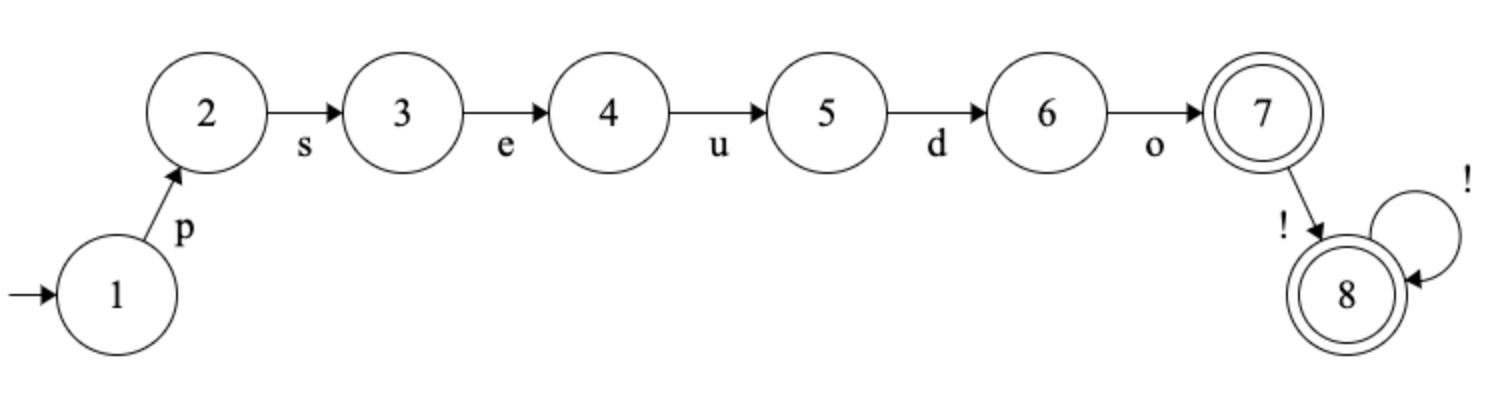
\includegraphics[scale=0.46]{assets/dfa.png}
    \caption{An example finite state automata.}
    \label{fig:dfa}
\end{figure}

Figure 2.1 shows an example of an FSA which accepts the word ``pseudo'' followed by an arbitrary number of exclamation marks. The FSA has 8 states, and the leftmost arrow indicates that \textbf{1} is the starting state. From here, we can get to the second state if our string starts with the symbol ``p''. Thus, all strings that do not begin with a ``p'' are rejected at this point. States 7 and 8 have an additional ring within their circle, which means that they are accepting states. If a combination of symbols have not been rejected at this point, and is finished, it is accepted. \hfill \\

State 8 has an arrow leading to itself via the symbol ``!'', meaning that it can end with as many exclamation marks as possible. A string like ``pseudo!!p!!!'' is not accepted, however, despite starting with ``pseudo!!'' and ending with ``!!!''. Once a string has reached state 8, it can \textit{only} be followed by exclamation marks, or else it is rejected. \hfill \\

Warren McCulloch and Walter Pitts were among the first researchers to introduce a concept similar to finite automata, all the way back in 1943~\cite{McCulloch43}. Their paper presents a simplified computational model of biological neurons. \hfill \\

There have been multiple attempts at creating flowchart editors, most notably by Carlisle et al.~\cite{carlisle2004} and Charntaweekhun et al.~\cite{charntaweekhun2006}. These allows authors to visualise their ideas, rather than keeping it all text based. Benefits of learning with help from visual aid is well documented. When it comes to computer science, visualisations are especially common in the context of machine learning \cite{ML_Visual1, ML_Visual2, ML_Visual3}. \hfill \\

One of few editors that generates flowcharts directly from code is Code2Flow\footnote{You can try the editor for free at \url{https://app.code2flow.com/}}. This is a DSL with support for most common programming concepts like statements, loops, conditionals, and more. The editor comes with a comprehensible guide on its syntax. It is also a highly customisable tool, letting you change the flowcharts' fonts, colours, sizes and even edge height. \hfill \\

\begin{figure}[ht]
\centering
\begin{subfigure}{.5\textwidth}
  \centering
  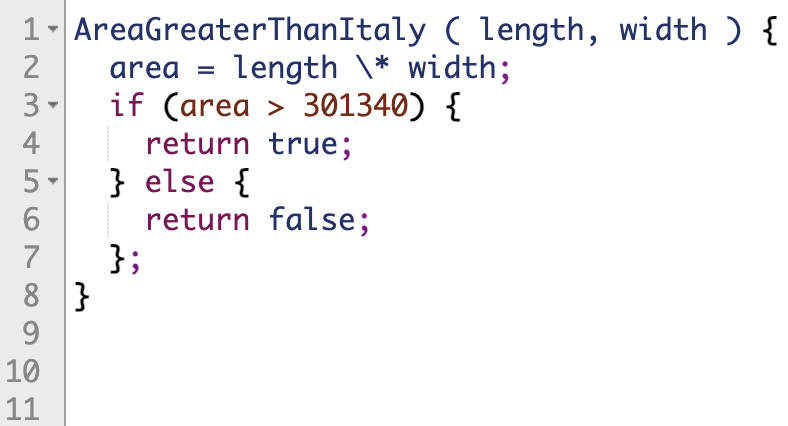
\includegraphics[width=1\linewidth]{assets/c2f_c.png}
  \caption{Code2Flow source code}
  \label{fig:c2f_code}
\end{subfigure}%
\begin{subfigure}{.3\textwidth}
  \centering
  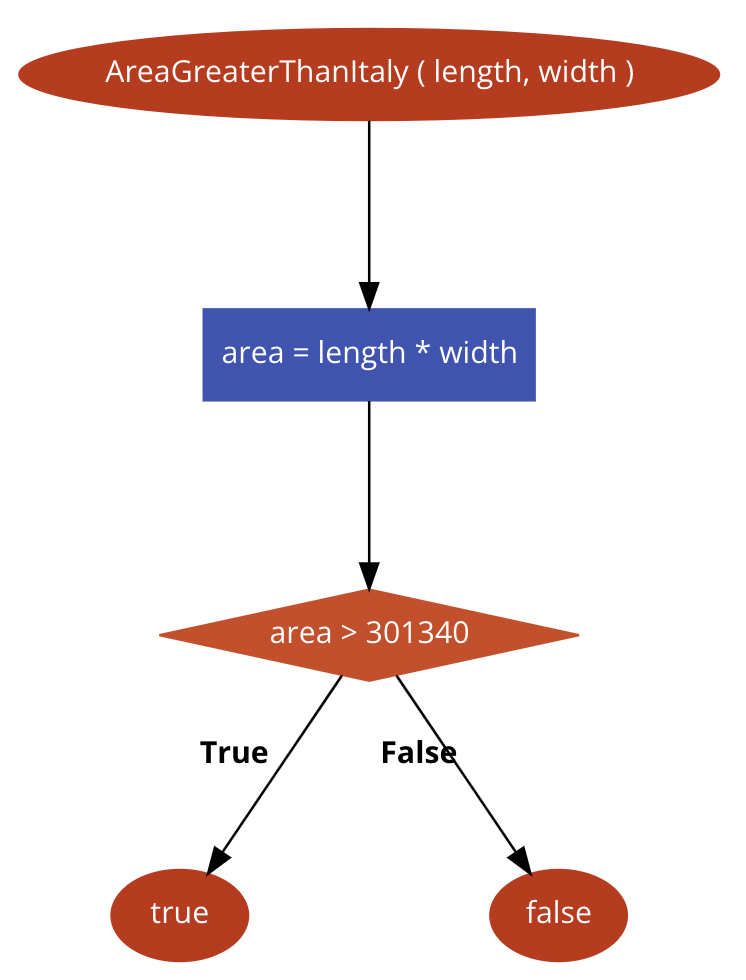
\includegraphics[width=1\linewidth]{assets/c2f_r.png}
  \caption{Compiled result}
  \label{fig:c2f_result}
\end{subfigure}
\caption{An algorithm written with Code2Flow, and the resulting flowchart}
\label{fig:AGTI_IBP}
\end{figure}

Given the imperative nature of flowcharts, the way they walk through problems step-by-step, there have also been attempts at converting flowcharts to pseudocode. Wu et al.~\cite{codeFromFlowcharts} proposed a structure identification algorithm, which can take an identified flowchart as input, and automatically generate code in return. This gives even more ground to perceive flowcharts as an image based form of pseudocode. \hfill \\

There have been multiple studies documenting the preference for flowcharts when it comes to studying algorithms, already back in the 80s by Scanlan et al.~\cite{DBLP:journals/software/Scanlan89} He documented how his students overwhelmingly preferred structured flowcharts to pseudocode for comprehending algorithms. Using multiple algorithms of varying complexity, the students most notably indicated that the flowcharts took less time to comprehend, provided fewer errors in understanding, and reduced the number of times they had to look at the algorithms. \hfill \\

More recently, Nita et al.~\cite{Nita_2020} attempted to analyse student's understanding of algorithms with pseudocode and flowcharts. The students were subjected to algol-like pseudocode and flowcharts. Their conclusion was that the students found it easier to understand the selected algorithms in image format, as compared to a text based approach.

% Bra språk for å snakke om flowcharts: https://www.researchgate.net/publication/234805404_Flowchart_techniques_for_structured_programming

\subsection{LaTeX}

LaTeX is a document preparation system that is widely used for the production of scientific documents\footnote{In fact, this thesis is written in LaTeX.}. It is an open-source typesetting system recognized for its capabilities in creating visually appealing documents that meet typographic standards. \hfill \\

LaTeX operates similarly to traditional programming, as it requires the user to write code to produce a document. The user typesets the document by typing commands in plain text, specifying the structure and styling of the content. This code is then compiled (see more in Section 2.2) to produce a formatted document, typically in PDF format. \hfill \\

This is a contrast to more ubiquitous word processors like Microsoft Word or Google Docs, which abide to WYSIWYG principles. This means that they display the final product as it is being edited, and allow users to manipulate the document directly through the GUI. \hfill \\

LaTeX builds upon the TeX typesetting system created by Donald Knuth. It added a collection of macros that simplified the use of TeX, and made it more accessible to non-technical users. \hfill \\

A distributed collection of macros in LaTeX is called a \textbf{package}. They allow users to add functionality or modify the behaviour of LaTeX, including refining typography, changing the layout of elements, creating graphics and more. In LaTeX documents, they are included using the \textbf{\textbackslash usepackage\{\}} command. \hfill \\

For this thesis, there are two LaTeX packages that are central: \textbf{Algorithm2e} and \textbf{TikZ}. Algorithm2e is a package to typeset algorithms or pseudocode. TikZ, on the other hand, is probably the most complex and powerful tool to create graphic elements in LaTeX. In this thesis, Algorithm2e will be used for pseudocode and TikZ for flowcharts. \hfill \\

%Algorithm2e provides an algorithm environment you can access through \\ \textbf{\textbackslash begin\{algorithm2e\}}\footnote{https://www.overleaf.com/learn/latex/Algorithms\#The\_algorithm2e\_package}. TikZ provides an environment you can access through \textbf{\textbackslash begin\{tikzpicture\}}\footnote{https://www.overleaf.com/learn/latex/TikZ\_package}. We must also remember to include \\ \textbf{\textbackslash usepackage\{algorithm2e\}} and \textbf{\textbackslash usepackage\{tikz\}} in our preamble. \hfill \\

\subsection{Examples}

Figure 2.3 shows how we can use the Algorithm2e package with LaTeX to write pseudocode. Figure 2.3 (a) shows the source code, and Figure 2.3 (b) shows the result of compiling said source coude. \hfill \\

The first lines show how algorithm2e can be loaded and cofigured. Some keywords must be declared, like \textbf{\textbackslash SetKwProg\{Prog\}\{Title\}} to denote title of our algorithm. \textbf{\textbackslash Prog} is what we write, and \textbf{Title} is what we see. Declaring a function keyword is optional, and all it really does is add a monospaced font. We can also opt to exclude semicolons. \hfill \\

We can add a description of input and output through \textbf{\textbackslash KwIn} and \textbf{\textbackslash KwOut}, respectively. We can also add a caption to the algorithm as a whole with \textbf{\textbackslash caption} at the end. \hfill \\

We can write the algorithm itself with natural language, but also utilise the embedded keywords of Algorithm2e. In the example we have used \textbf{\textbackslash uIf}, \textbf{\textbackslash uElse} and \textbf{\textbackslash Return}, as well as mathematical symbols like $\gets$ and $\cdot$ by wrapping them in dollar signs. \newpage % forsiktig med denne kommandoen

\begin{figure}[ht]
\centering
\begin{subfigure}{.8\textwidth}
  \centering
  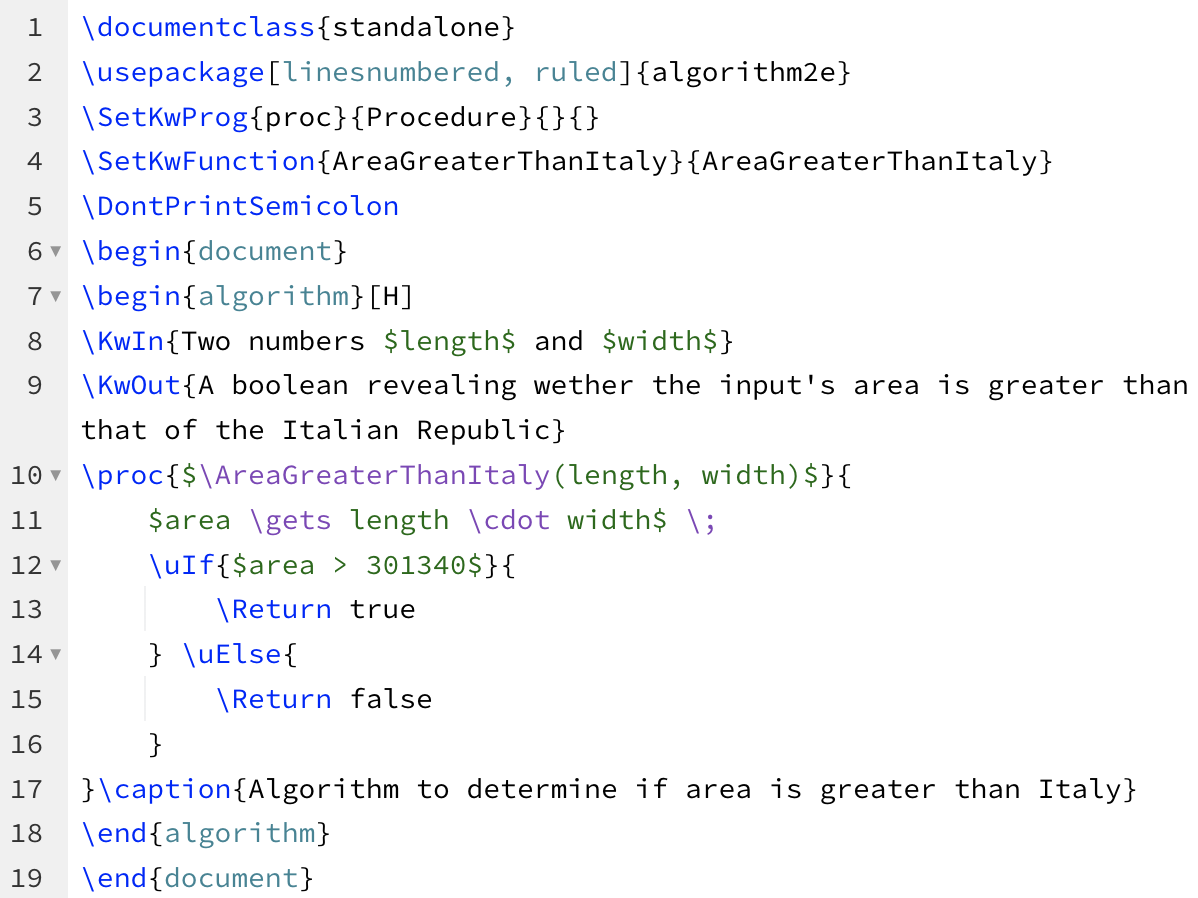
\includegraphics[width=1\linewidth]{assets/AGTI_TBP_s.png}
  \caption{LaTeX source code}
  \label{fig:AGTI_TBP_source_code}
\end{subfigure} \newline

\begin{subfigure}{.8\textwidth}
  \centering
  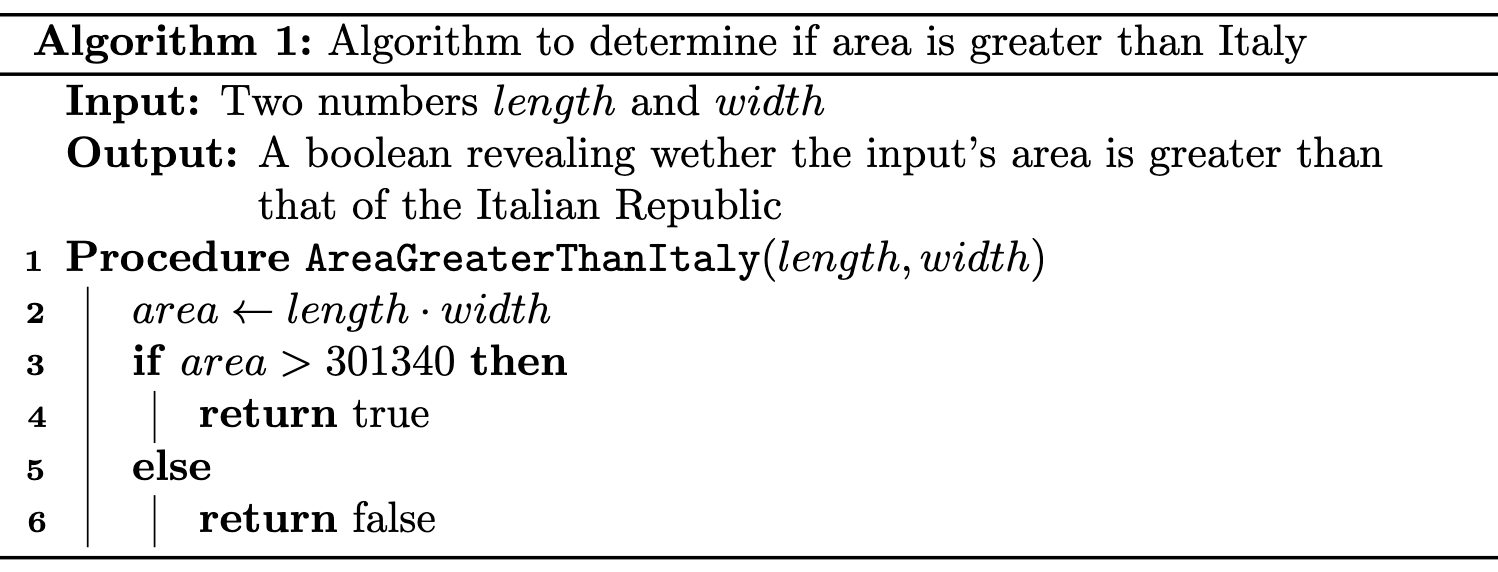
\includegraphics[width=1\linewidth]{assets/AGTI_TBP.png}
  \caption{Compiled result}
  \label{fig:AGTI_TBP_result}
\end{subfigure}
\caption{A program written in LaTeX, using the Algorithm2e package}
\label{fig:AGTI_TBP}
\end{figure}

Figure 2.4 shows how we can use the TikZ with LaTeX to draw flowcharts. Figure 2.4 (a) shows the source code, and Figure 2.4 (b) shows the result of compiling said source coude. \hfill \\

Again, the first lines show how the package can be loaded and configured. After loading TikZ, we specify what we want to use from the package, which in this case is \textbf{shapes} and \textbf{arrows}. We also specify the node distance, in centimeters. \hfill \\

Flowcharts with TikZ are constructed in three primary steps:

\begin{enumerate}
    \item Defining the style of nodes and edges
    \item Declaring the nodes
    \item Declaring the edges
\end{enumerate}

Each node style has a label and a shape, along with more specific metadata like height and colour. When declaring nodes in the next step, we give them an identifier, a style and the text which occurs in them. When declaring edges, we can simply point out the style, the child and the parent. Each edge must be drawn individually. In this example the edges have direction, but this can be changed by omitting the \texttt{->} option on line 10.

\begin{figure}[ht]
\centering
\begin{subfigure}{.7\textwidth}
  \centering
  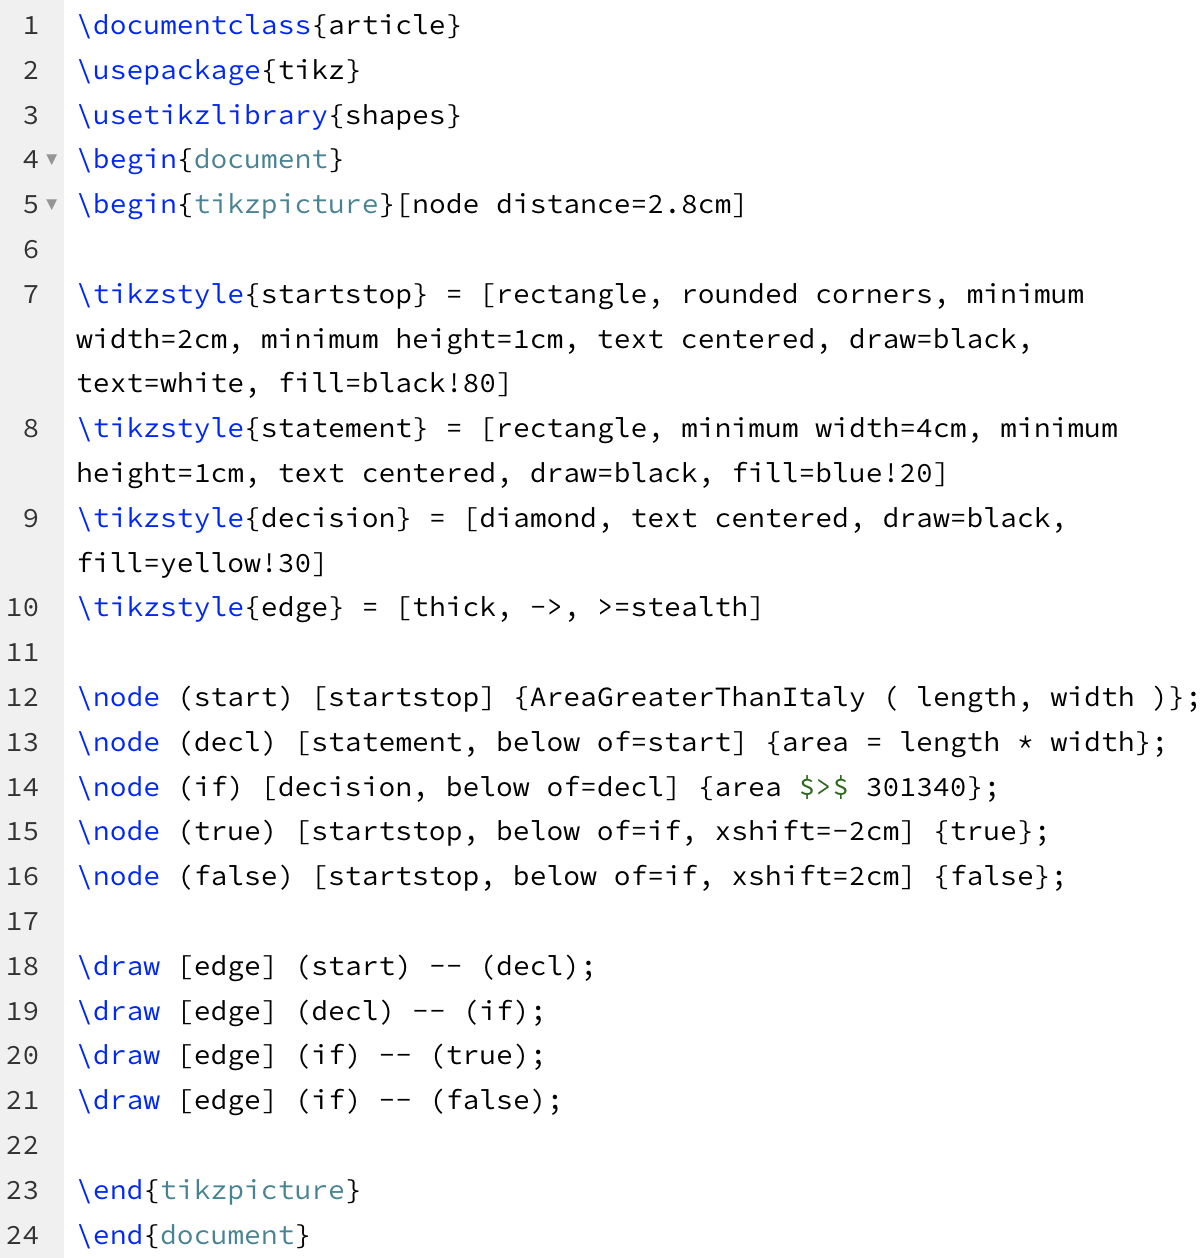
\includegraphics[width=1\linewidth]{assets/AGTI_IBP_s.png}
  \caption{LaTeX source code}
  \label{fig:AGTI_IBP_source_code}
\end{subfigure} \newline

\begin{subfigure}{.4\textwidth}
  \centering
  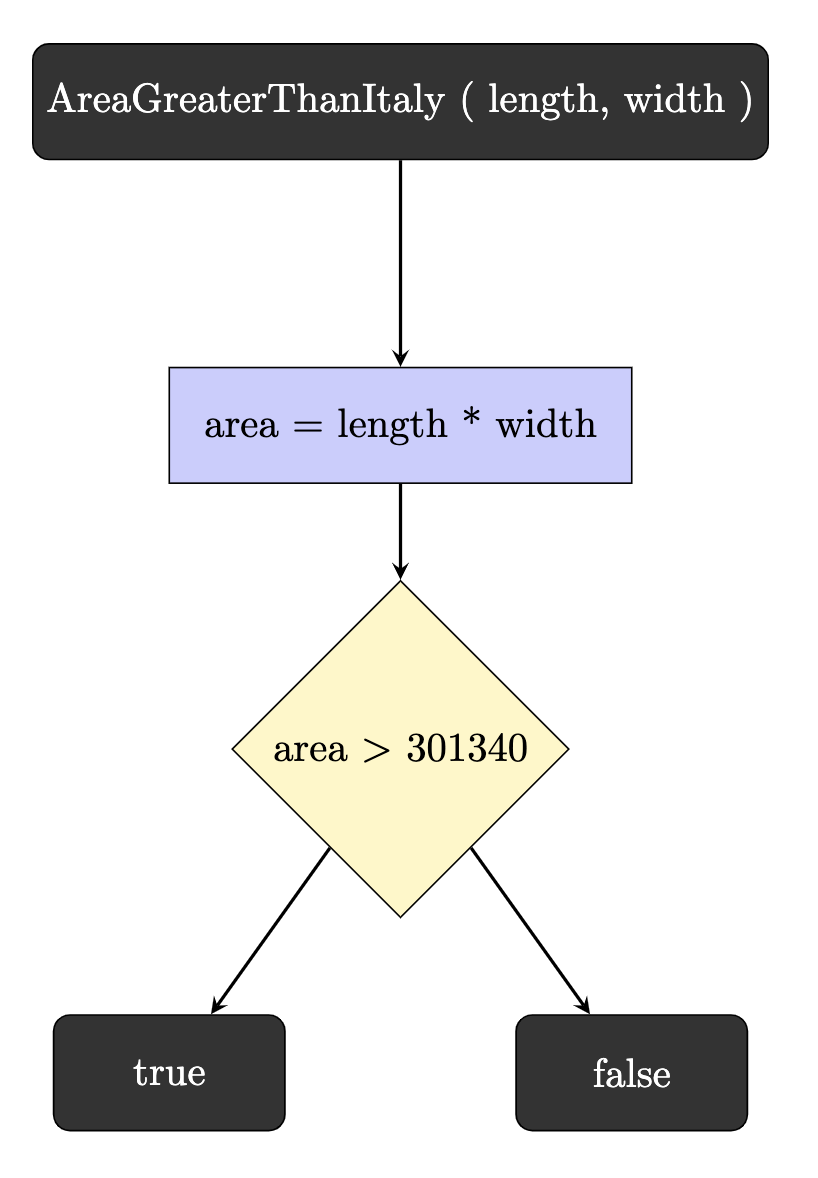
\includegraphics[width=.4\linewidth]{assets/AGTI_IBP.png}
  \caption{Compiled result}
  \label{fig:AGTI_IBP_result}
\end{subfigure}
\caption{A program written in LaTeX, using the TikZ package}
\label{fig:AGTI_IBP}
\end{figure}

\section{Haskell}

As previously mentioned, we opted for the Haskell programming language to implement Psnodig. Knowing the ins and outs of Haskell is not crucial for understanding the thesis. However, there are some aspects of the language that are key to the implementation, and majority of the provided listings in this thesis will be in Haskell. \hfill \\

\subsection{Data types}

Types in Haskell are also called \textbf{data types}, as the \textbf{type} keyword is used to create type aliases. \hfill \\

A common type in any programming language is the boolean, shown in Listing 2.1. All types have one or more \textbf{value constructors}, which specify the different values a certain type can have. In this case, the Boolean type can have one of two values: True or False. The pipe operator functions as an ``or'' \cite[be stian om å sjekke hvilken side dette eksemplet er på i boka]{LYAH}. \hfill \\

\begin{lstlisting}[caption={Recreating the Boolean data type with Haskell}, captionpos=b]
    data Boolean = False | True
\end{lstlisting}

With Haskell, it is straightforward to create your own data types, which can then be used to model ASTs. For instance, we can create our own calculator language in just a few lines of code, as shown in Listing 2.2. \hfill \\

\begin{lstlisting}[caption={Example data types in Haskell}, captionpos=b]
    data Program = Program Expression

    data Expression =
          CompoundExpression Integer Operator Expression
        | IntExpression Integer

    data Operator =
          Plus
        | Minus
        | Times
        | Division
\end{lstlisting}

From this, we can construct an AST as the one we see in Listing 2.3. \hfill \\

\begin{lstlisting}[caption={An AST constructed with data types presented in Listing 2.2}, captionpos=b]
    Program (CompoundExpression 1 Plus
                (CompoundExpression 2 Minus
                    (IntExpression 3))
\end{lstlisting}

Naturally, we could create much bigger calculations than this. If we wish to expand our operators data type, we only have to add a pipe and the operator name, as shown in Listing 2.4. \hfill \\

\begin{lstlisting}[caption={An extended version of the Operator data type presented in Listing 2.2}, captionpos=b]
    data Operator =
          Plus
        | Minus
        | Times
        | Division
        | Exponent
\end{lstlisting}

\subsection{Pattern matching}

Another integral part of Haskell, is that its strong type system opens for clean and efficient pattern matching. This is a very useful method for deconstructing and working with data, and for making decisions based on the data's shape. \hfill \\

Pattern matching is demonstrated in Listing 2.5, with a function converting each value of the Operator type (introduced in Listing 2.2) to its string equivalent. It shows a function \texttt{convert} that takes a value of type Operator as input, and returns a value of type String. \hfill \\

\begin{lstlisting}[caption={Haskell function converting values of one type to another}, captionpos=b]
    convert :: Operator -> String
    convert Plus     = " + "
    convert Minus    = " - "
    convert Times    = " / "
    convert Division = " * "
\end{lstlisting}

If the function shown in Listing 2.5 was to work on the extended Operator data type from Listing 2.4, the compiler would let us know that our pattern matching is in, as there is no case for the \texttt{Exponent} value. This is one of the features that make pattern matching so powerful and safe. For some types though, like \texttt{Integer}, it can be exhausting to define injective functions. Listing 2.6 shows how the underscore can be used to capture all remaining values of a type. \hfill \\

\begin{lstlisting}[caption={A simple Haskell function converting values of type Integer to its string equivalent}, captionpos=b]
    convertInt :: Integer -> String
    convertInt 1 = "one"
    convertInt 2 = "two"
    convertInt _ = "in integer other than one or two"
\end{lstlisting}

\subsection{Testing}

Lastly, Haskell allows us to utilise the QuickCheck, which is a testing library suited for automatic property-based testing.\footnote{Full documentation can be found at \url{https://hackage.haskell.org/package/QuickCheck}} QuickCheck can be used to prove various properties of our tool~\cite{DBLP:conf/icfp/ClaessenH00}.

\section{Compilers}

A compiler is, in simple terms, a tool that reads a program in a high-level language and translates it to an executable target program~\cite{DBLP:books/aw/AhoSU86}. It consists of a frontend and a backend. The frontend is often referred to as the analysis part, whilst the backend is referred to as the synthesis part. \hfill \\

\begin{figure}[ht]
    \centering
    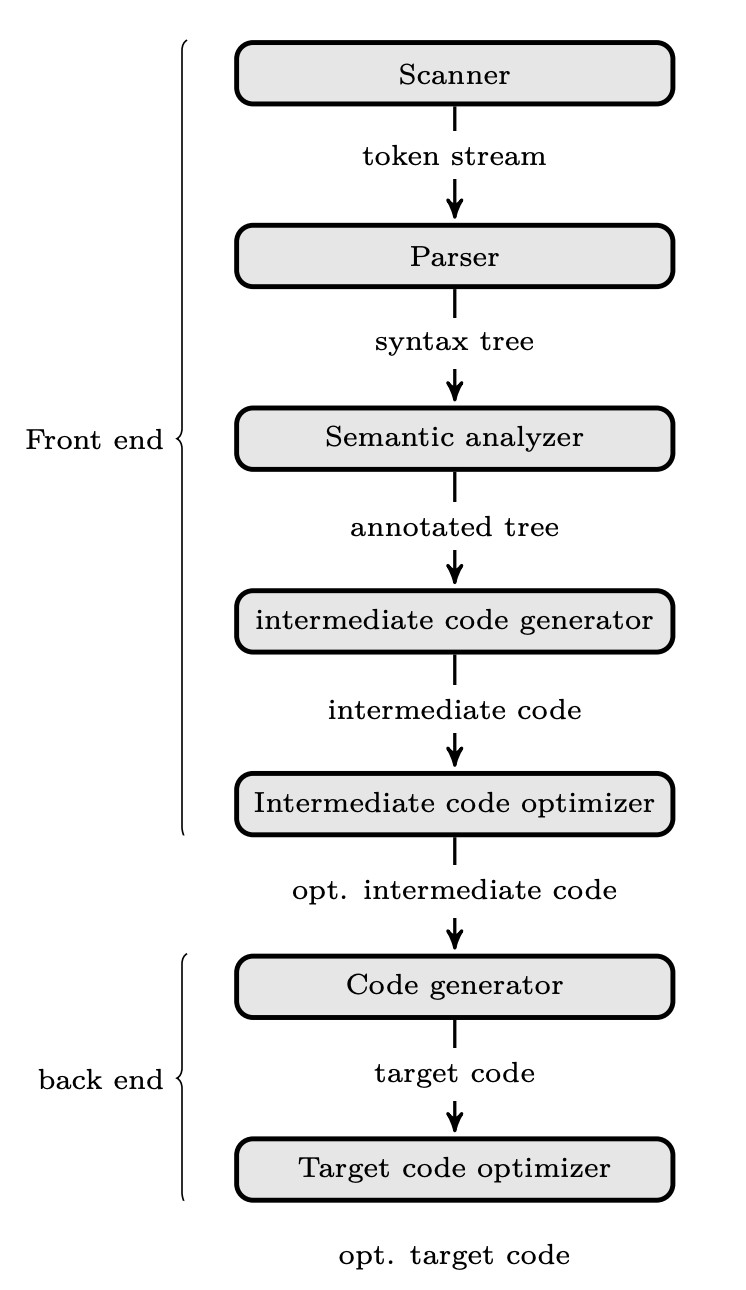
\includegraphics[scale=0.35]{assets/compilerOutline.png}
    \caption[]{The phases of a typical compiler.\footnotemark}
    \label{fig:compilerOutline}
\end{figure}
\footnotetext{The image is borrowed by Martin Steffen's script on compiler construction: \url{https://www.uio.no/studier/emner/matnat/ifi/INF5110/v24/script/}}

The frontend of a compiler is responsible for reading the character stream of a source program, and converting them into appropriate tokens. These tokens are then used to create an intermediate representation of the source program. It is during the analysis part that a compiler will detect a program's syntactic errors, if there are any. \hfill \\

Often, the analysis part involves a symbol table, which maintains information about syntactic entities of the source program. This is passed along with the intermediate representation to the synthesis part, for optimisation reasons. Common entities are bindings and typing. \hfill \\

The backend of a compiler is responsible for producing the desired target program from the intermediate representation. This target program is intended to be executable. For instance, source code written in C is compiled down to an executable binary.

\subsection{Transpilers}

A transpiler, formally \textbf{source-to-source compiler}, is a tool that converts input source code into output source code, whilst maintaining a similar abstraction level~\cite{DBLP:conf/els/MarcelinoL22}. The first transpiler to our knowledge was developed in 1978 by Intel, with the aim of translating assembly source code from the 8080/8085 processor to the 8086 processor~\cite{intel1979}. \hfill \\

The JavaScript programming language\footnote{\url{https://developer.mozilla.org/en-US/docs/Web/JavaScript/Language_overview}} has a rich history of transpiling.
% It is the most common programming language for working on the web.\footnote{\url{https://survey.stackoverflow.co/2023/#most-popular-technologies-language}} \\
As a language in constant development, it faces the issue where not all browsers are always compatible with its newest features. Therefore, there exists a transpiler Babel\footnote{\url{https://babeljs.io}} which converts modern JavaScript into a backwards compatible version. According to Nicolini et al.~\cite{DBLP:journals/software/NicoliniHF24}, without a transpiler almost 14\% of web users risk facing a JavaScript bug when accessing a website with new JavaScript features. \hfill \\

Not only JavaScript can be transpiled to JavaScript. In fact, the list of other programming languages and tools that can be transpiled to JavaScript is so extensive that it is potential for its own thesis.\footnote{\url{https://gist.github.com/matthiasak/c3c9c40d0f98ca91def1} provides a list of 320 languages and tools that compile to JavaScript.} However, we can bring forward a few notable exambles. \hfill \\

Unlike JavaScript, TypeScript is structurally typed. TypeScript is syntactically a superset of JavaScript, as it adds a static typing layer. The primary purpose of these types is to enhance the development experience by catching potential errors during compilation, and making the code more maintainable. However, before the code is run, TypeScript is transpiled into plain JavaScript, and the types are stripped away \cite{TypeScript}. \hfill \\

AlaSQL is an open-source SQL database for JavaScript.\footnote{\url{https://github.com/AlaSQL/alasql}} It is technically a transpiler since we work in a JavaScript environment, but it allows you to write CRUD operations in SQL, like displayed in Listing 2.1.

\begin{lstlisting}[caption={JavaScript code to create, populate and select a table with AlaSQL}, captionpos=b]
    alasql("CREATE TABLE
            cities (city string, pop number)");

    alasql("INSERT INTO cities
            VALUES ('Paris', 2249975),
                   ('Berlin', 3517424),
                   ('Madrid', 3041579)");

    const res = alasql("SELECT *
                        FROM cities
                        WHERE pop < 3500000
                        ORDER BY pop
                        DESC");
\end{lstlisting}

Despite all the commands being written in SQL, \texttt{res} has a JavaScript value of a list with two objects, as seen in Listing 2.2.

\begin{lstlisting}[caption={JSON list with two objects}, captionpos=b]
    [
        {
            "city": "Madrid",
            "pop": 3041579
        },
        {
            "city": "Paris",
            "pop": 2249975
        }
    ]
\end{lstlisting}

\forsup{Ett til eksempel med JS?}

\forsup{\url{https://ieeexplore.ieee.org/abstract/document/9930246/references\#references} refererer til AlaSQL-githuben som en kilde, istedenfor fotnote. Kan jeg gjøre det samme? Bør fotnoter egentlig bare være digresjoner og sånt?}

Transpilation is not exclusive to JavaScript, however. It is a common practice in many other programming languages that must interact with or be portable across diverse systems. For instance, Haskell uses GHC (Glasgow Haskell Compiler) to compile its code, which at one point converted its code into C rather than direct generation of native code. This enabled Haskell to run on any platform with a C compiler. It also benefits directly from others' improvements in C code generation \cite{HaskellToC}. \hfill \\

Another example is a transpiler presented by Lunnikiv et. al~\cite{DBLP:conf/samos/LunnikiviJ020}, where Python is converted to Rust as an intermediate source code step. The paper shows how pre-existing Python implementations that depend on optimised libraries can be transpiled to Rust semi-automatically. This way, the user can keep writing Python, whilst additionally allowing for the performance optimisation given by Rust.

\subsection{Parsers and code generators}

We remember that the frontend of a compiler is tasked with reading source code, and --- given that it is syntactically correct --- build an intermediate representation. The backend of a compiler is tasked with converting that intermediate representation into target code. \hfill \\

Having in depth knowledge about the entire pipeline of a compiler is not necessary to understand the rest of the thesis. However, the first and the last parts of a compiler will be central topics. Specifically I am referring to the parser and the code generator. \hfill \\

These two play a vital role in a transpiler. In fact, they are all you really need to build a simple transpiler (in addition to a defined intermediate representation). When the parser has converted the source code to an intermediate representation, the code generator can convert that intermediate representation into target code. Given the fact that even the simplest language could write infinitely many different programs, we must lean on some kind of intermediate representation. \hfill \\

Technically, the parser and the code generator are completely independent from one another. The only thing they must have in common is the ability to read/write the same intermediate representation. There are several advantages to this, like flexibility and modularity. If we want our transpiler to read or write another language, we can just create an additional parser or code generator. When we add a parser, we do not have to do any changes to our code generator, and vice versa, because they work on the same intermediate representation, independent of how the source- and target programs look like. \hfill \\

An example of this is the programming language \textbf{Derw}, an ML language mainly inspired by Elm.\footnote{\url{https://github.com/eeue56/derw}} Its compiler can only parse Derw code, however it comes with multiple code generators (referred to as just ``generators'') which as of writing this target JavaScript, TypeScript, Elm and even English and Derw itself. As it is open sourced, anyone can fork the repository and add their own code generator, if they wish. \hfill \\

Listing 2.3 shows how expressions like $6 <= 8$ are converted. The token \textbf{lessThanOrEqual} has a left- and right pointer, corresponding to the respective integers. These are extracted, and put on each side of the string ``is less than or equal to''.\footnote{The entire English code generator can be found at \url{https://github.com/eeue56/derw/blob/main/src/generators/English.derw}} \hfill \\

\begin{lstlisting}[caption={The function that converts a ``less than or equal''-expression in Derw to English}, captionpos=b]
    generateLessThanOrEqual: LessThanOrEqual -> string
    generateLessThanOrEqual lessThanOrEqual =
        let
            left: string
            left =
                generateExpression lessThanOrEqual.left

            right: string
            right =
                generateExpression lessThanOrEqual.right
        in
            `$\textdollar${left} is less than or equal to $\textdollar${right}`
\end{lstlisting}

Another example is \textbf{Pandoc}, which is a software that converts between different markdown formats~\cite{dominici2014}. It includes a Haskell library, as well as a command-line program. It is able to a document from 45 source formats to 63 target formats.\footnote{See the entire list at \url{https://hackage.haskell.org/package/pandoc}} Additionally, Pandoc is able to convert documents in LaTex, Groff ms and HTML into PDFs. \hfill \\

At its core, Pandoc is really just an abstract syntax tree (AST) of Haskell data types. A Pandoc document has the type \textbf{Pandoc Meta [Block]}. The first attribute is \textit{Meta}, metadata for the document, like its title, its author(s), the date it was written and more. The second attribute is a list of \textit{Block}. A block is a more intricate data type, which is shown in its entirety in Listing 2.4.

\begin{lstlisting}[caption={The ``Block'' data type of Pandocs native representation}, captionpos=b]
    Plain [Inline]
    Para [Inline]
    LineBlock [[Inline]]
    CodeBlock Attr String
    RawBlock Format String
    BlockQuote [Block]
    OrderedList ListAttributes [[Block]]
    BulletList [[Block]]
    DefinitionList [([Inline], [[Block]])]
    Header Int Attr [Inline]
    HorizontalRule
    Table [Inline] [Alignment] [Double] [TableCell] [[TableCell]]
    Div Attr [Block]
    Null    
\end{lstlisting}

The modular design of Pandoc means that adding an input or output formats only requires adding a program that can convert \textit{to} this native representation, and a program that can convert \textit{from} this native representation. This is much like parsers and code generators of compilers, but as they are much less intricate, the Pandoc documentation refers to them simply as \textbf{readers} and \textbf{writers}. \hfill \\

However, writing a document in a rich format like Latex, and later converting it to a different markup language might tends to pose problems due to the different philosophies that underlie each language. As the native representation is less expressive than many of the formats it converts between, the user cannot always expect perfect conversions. Yet Pandoc is an excellent interpreter of lightweight markup languages like Markdown, which are ``neutural'' by design~\cite{dominici2014}. \hfill \\

An example of conversion with Pandoc is provided in Figure 2.6. The input format is Markdown, and the output format is LaTeX. Figure 2.6 (b) shows the intermediate, native representation in Haskell. Meta contains title and date, while the list entries in Block are of type Header and Para. \hfill \\

\begin{figure}[ht]
\centering
\begin{subfigure}{.6\textwidth}
  \centering
  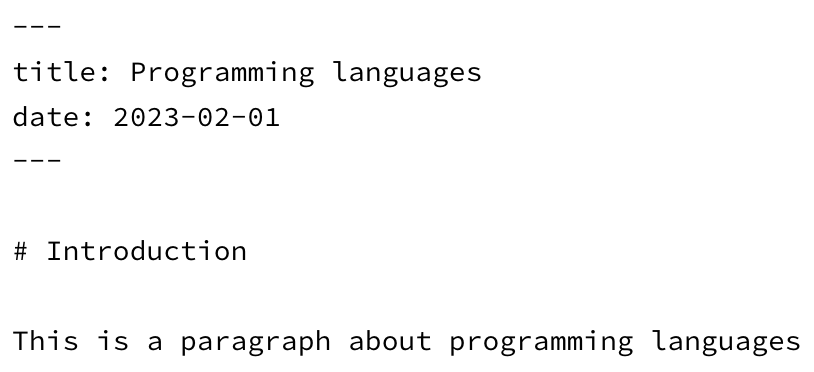
\includegraphics[width=1\linewidth]{assets/pandocMD.png}
  \caption{A Markdown program}
  \label{fig:a}
\end{subfigure}
\begin{subfigure}{.6\textwidth}
  \centering
  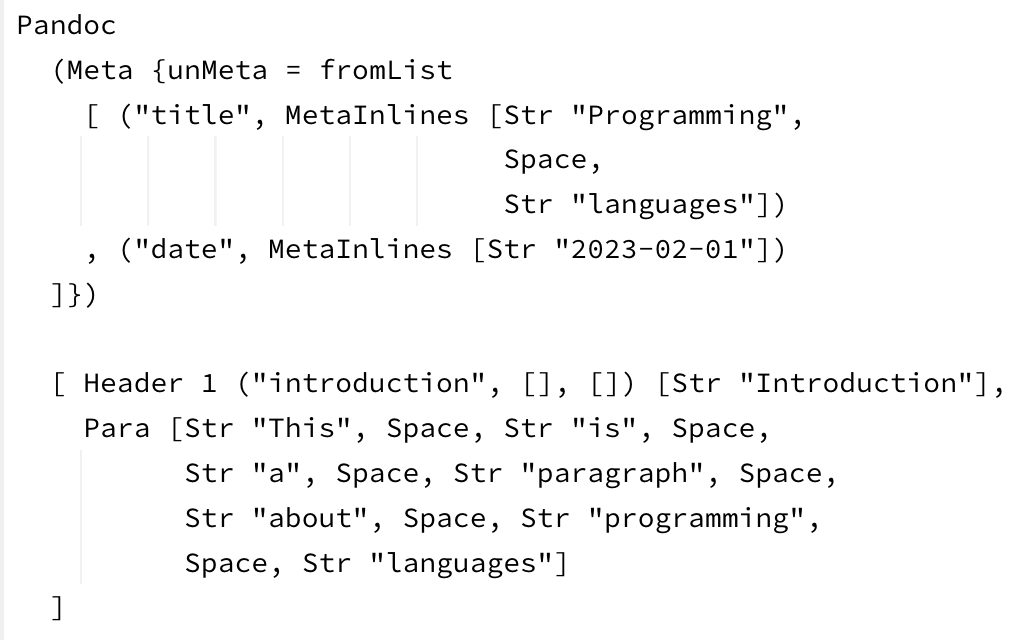
\includegraphics[width=1\linewidth]{assets/pandocHASKELL.png}
  \caption{The internal Pandoc AST of (a)}
  \label{fig:b}
\end{subfigure}
\begin{subfigure}{.6\textwidth}
  \centering
  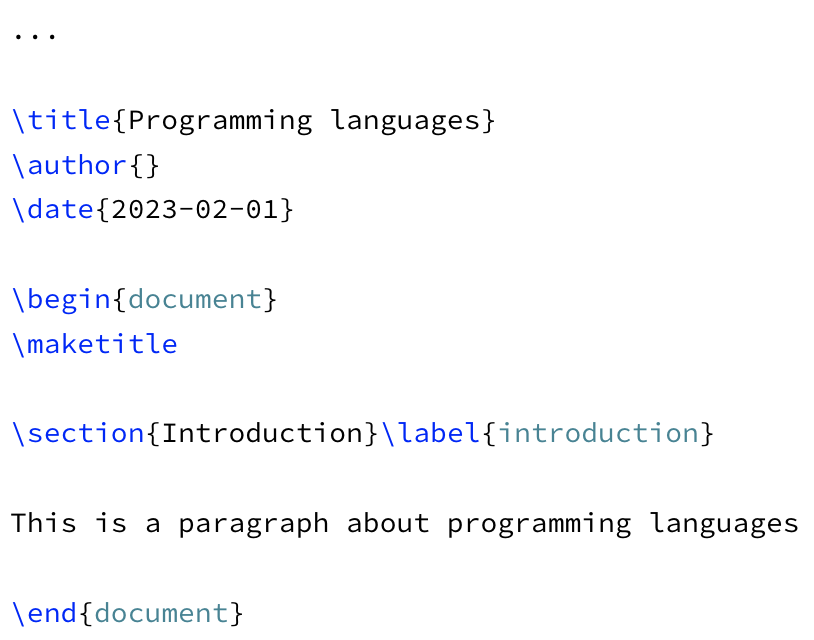
\includegraphics[width=1\linewidth]{assets/pandocLATEX.png}
  \caption{A LaTeX program, built from the AST in (b)}
  \label{fig:c}
\end{subfigure}

\caption{A Markdown program converted to LaTeX with Pandoc}
\label{fig:d}
\end{figure}